\chapter{Instalación de Certificados en Thunderbird e Intercambio de Correo S/MIME}

\section{Instalación del certificado raíz}
\subsection{Enunciado:}
1.2.1. Una vez creado nuestro certificado digital, hemos de configurar el cliente de correo electrónico
Mozilla Thunderbird para que pueda firmar y cifrar mensajes con dicho certificado. Los correos a través de
web (como el de la ULPGC) no permiten el uso de certificados, así que si no lo tenemos instalado, habrá que
configurar previamente Mozilla Thunderbird con nuestro correo electrónico personal (no el de la ULPGC).


El primer paso es importar la parte pública del certificado raíz (\texttt{certificadoRaiz.crt}) en Mozilla Thunderbird para que el cliente de correo confíe en los certificados firmados por esta CA.

En Thunderbird, se accede a \textbf{Herramientas $\rightarrow$ Opciones $\rightarrow$ Avanzado $\rightarrow$ Administrar certificados} (o \textbf{Ajustes $\rightarrow$ Privacidad y seguridad $\rightarrow$ Gestionar certificados}).

Al importar el certificado raíz se le asigna confianza para \textit{identificar direcciones de correo electrónico}. El certificado aparece en la pestaña \textbf{Autoridades}, bajo la organización ``ULPGC -- Seguridad de la Información''.

\begin{figure}[H]
    \centering
    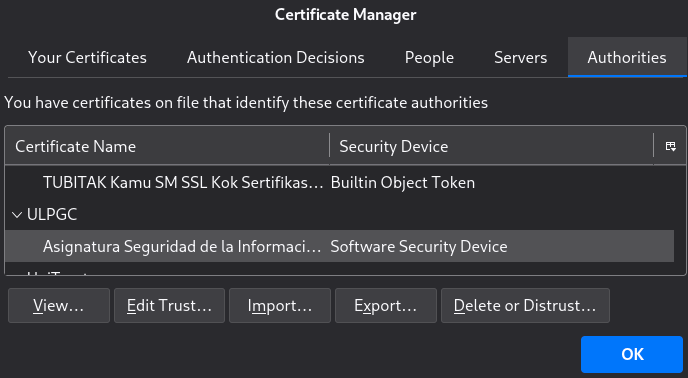
\includegraphics[width=\textwidth]{Imagenes/1.2.2.png}
    \caption{Importación del certificado raíz en Thunderbird (almacén de Autoridades)}
    \label{fig:importar_raiz}
\end{figure}

\section{Instalación del certificado personal}
\subsection{Enunciado:}
1.2.2. En este cliente de correo electrónico hemos de instalar tanto la parte pública del certificado raíz
(fichero \texttt{certificadoRaiz.crt}), como nuestro certificado personal completo (fichero
\texttt{certificadoPersonal.p12}) con la contraseña que le pusimos. En Thunderbird, hay que acceder a
Herramientas/Opciones/Avanzado/Administrar certificados). Al Importar el certificado raíz, asignarle
confianza para gestionar correo electrónico y verificar que se encuentra en el almacén de ``Autoridades''
(debe aparecer en primer lugar, ya que el nombre de la organización es ``ULPGC -- Seguridad de la
Información''. A continuación, hemos de importar nuestro \texttt{certificadoPersonal.p12} e introducir la
contraseña que lo protege. Verificar que nuestro certificado personal aparece en el almacén de ``Sus
certificados'' o similar.

A continuación se importa el fichero \texttt{certificadoPersonal.p12} que contiene tanto la clave privada como el certificado personal. Thunderbird solicita la contraseña de protección del \texttt{.p12} que establecimos anteriormente.

Tras la importación, nuestro certificado aparece en la pestaña \textbf{Sus certificados}.

\begin{figure}[H]
    \centering
    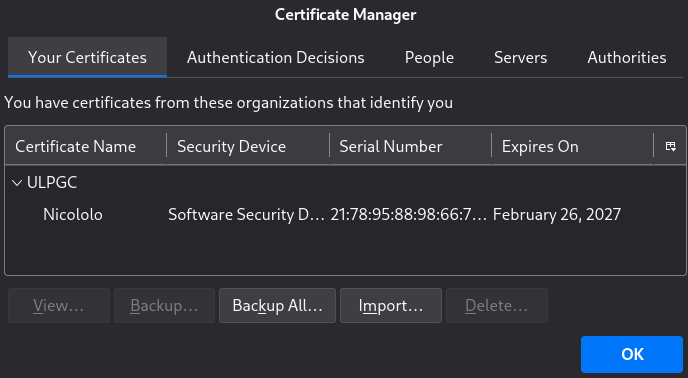
\includegraphics[width=\textwidth]{Imagenes/1.2.1.png}
    \caption{Certificado personal importado en Thunderbird (pestaña ``Sus certificados'')}
    \label{fig:importar_personal}
\end{figure}

\section{Configuración de la cuenta de correo}
\subsection{Enunciado:}
1.2.3. Con ambos certificados ya instalados, hay que configurar nuestra cuenta de correo electrónico para
que utilice nuestro certificado personal, en Thunderbird eso se hace en Herramientas/Configuración de
cuenta/Seguridad\dots al pulsar el botón de Seleccionar en las opciones de Firmado Digital y Cifrado debe
aparecer seleccionado nuestro certificado personal que cargamos previamente. Importante: no seleccionar
las opciones de firmar y cifrar siempre, es mejor decidir cuándo se envían mensajes firmados y cifrados
antes de enviar cada mensaje.

Para que Thunderbird utilice nuestro certificado al firmar y cifrar mensajes, se configura la cuenta:

\begin{enumerate}
    \item Acceder a \textbf{Herramientas $\rightarrow$ Configuración de cuenta $\rightarrow$ Cifrado de extremo a extremo} (o \textbf{Seguridad} en versiones anteriores).
    \item En la sección de \textbf{S/MIME}, pulsar \textit{Seleccionar} tanto para \textbf{Firmado digital} como para \textbf{Cifrado}.
    \item Seleccionar nuestro certificado personal en ambos casos.
    \item \textbf{Importante:} No marcar las opciones de firmar y cifrar siempre por defecto; es preferible decidir para cada mensaje individualmente.
\end{enumerate}

\section{Intercambio de certificados con la compañera}
\subsection{Enunciado:}
1.2.4. Una vez configurado e instalado el certificado, podremos FIRMAR los mensajes que enviemos, pero
para cifrar correo hacia un destinatario, es necesario disponer previamente de SU certificado personal
(obviamente, sólo con la clave pública). Por tanto aconsejamos intercambiar mensajes SOLO FIRMADOS
con otro compañero y así nuestro programa de correo almacenará el certificado del compañero que acompaña
a su mensaje cifrado. Una vez que verifiquemos que el certificado del compañero está en nuestro almacén de
``Otras personas'', ya podremos intercambiar mensajes cifrados y firmados.

Para poder enviar correo cifrado a un destinatario, es necesario disponer previamente de su certificado (clave pública). El procedimiento de intercambio es:

\begin{enumerate}
    \item \textbf{Enviar un mensaje solo firmado} a la compañera (Wafa Azdad Triki). Al firmar, se adjunta automáticamente nuestro certificado público.
    \item La compañera recibe el mensaje firmado y Thunderbird almacena nuestro certificado en el almacén de \textbf{Otras personas}.
    \item La compañera nos envía un mensaje firmado a nosotros o con su certificado adjunto, como en este caso, de modo que recibimos su certificado.
    \item Verificar que el certificado del compañero aparece en \textbf{Otras personas} en el administrador de certificados.
\end{enumerate}

\subsection{Envío de mensaje firmado}

Se compone un mensaje con el asunto ``Nicolás Rey Alonso'' dirigido a la compañera, activando la opción de \textbf{firma digital} (sin cifrado, ya que aún no tenemos su certificado):

\begin{figure}[H]
    \centering
    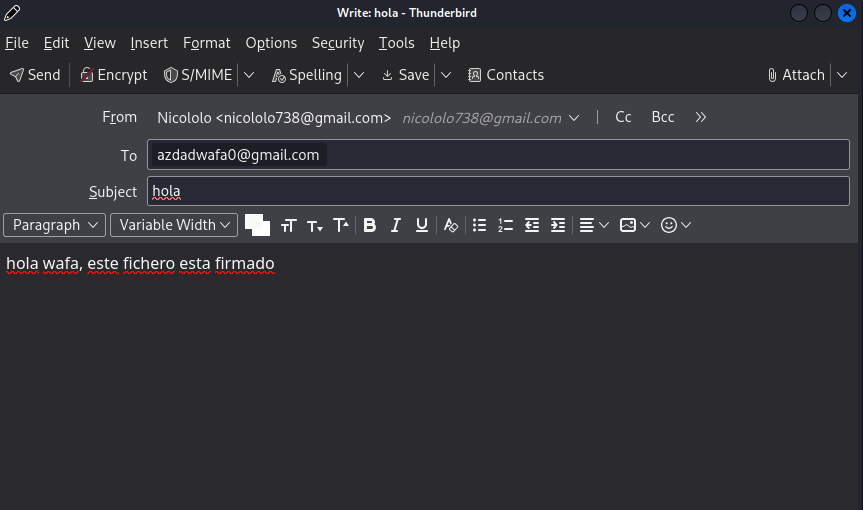
\includegraphics[width=\textwidth]{Imagenes/Correo_Firmado_Por_Mi_thunderbird1.png}
    \caption{Composición de mensaje firmado digitalmente}
    \label{fig:correo_firmado_1}
\end{figure}

\begin{figure}[H]
    \centering
    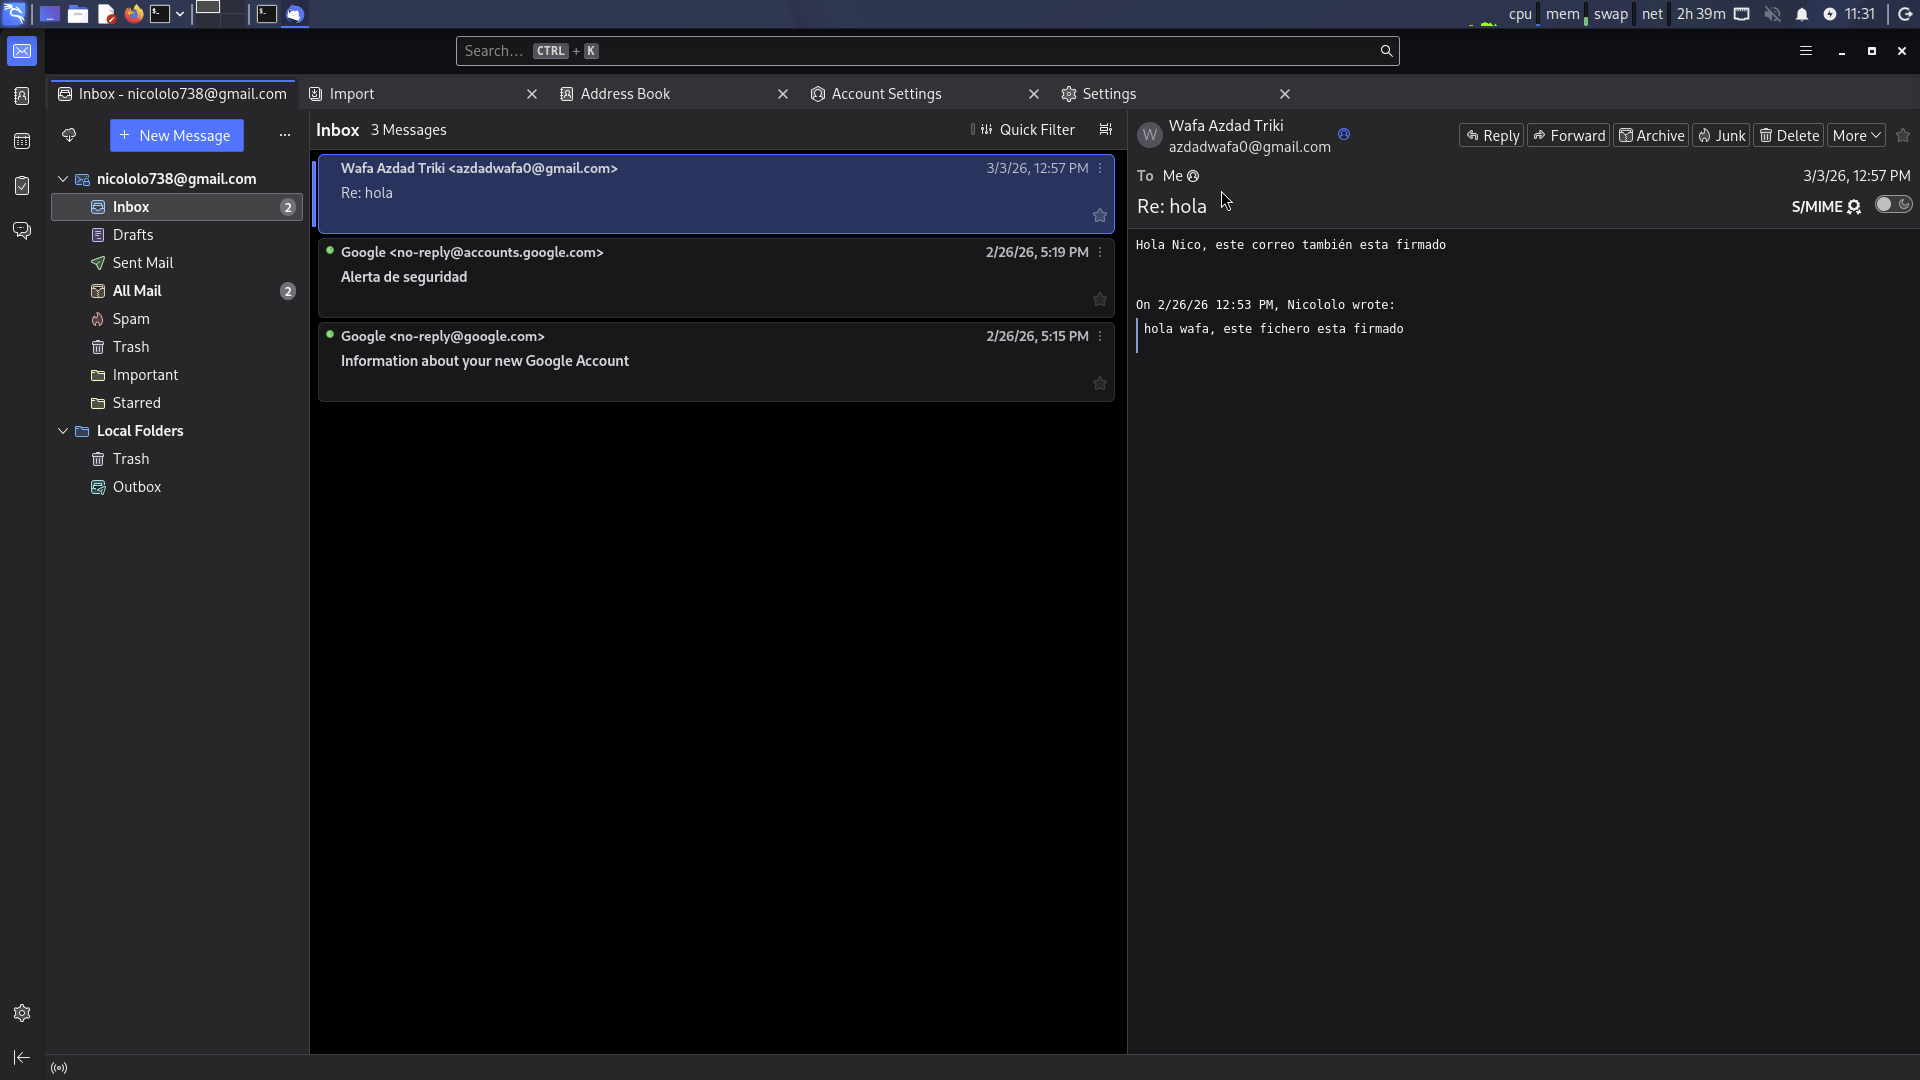
\includegraphics[width=\textwidth]{Imagenes/Correo_Firmado_Por_Mi_thunderbird2.png}
    \caption{Mensaje firmado enviado correctamente}
    \label{fig:correo_firmado_2}
\end{figure}

\subsection{Certificado de la compañera en Thunderbird}

Tras recibir un mensaje firmado por la compañera, su certificado queda almacenado en Thunderbird:

\begin{figure}[H]
    \centering
    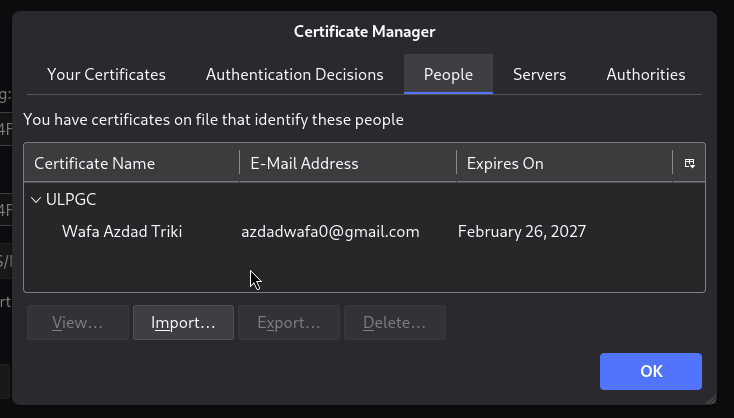
\includegraphics[width=\textwidth]{Imagenes/Certificado_Wafa_thunderbird.png}
    \caption{Certificado de Wafa Azdad Triki en el almacén de Thunderbird}
    \label{fig:cert_wafa}
\end{figure}

\section{Envío de mensaje cifrado y firmado}
\subsection{Enunciado:}
1.2.5. Enviar un mensaje con Asunto: (nombre y apellidos) a dicha dirección de correo (la del compañero)
con un breve texto de salutación y sobre todo, con las opciones de firmado y cifrado activadas.

Una vez que disponemos del certificado de la compañera, podemos enviar un mensaje tanto \textbf{firmado} como \textbf{cifrado}. El cifrado se realiza con la clave pública del destinatario, de modo que solo él puede descifrarlo con su clave privada.

\begin{figure}[H]
    \centering
    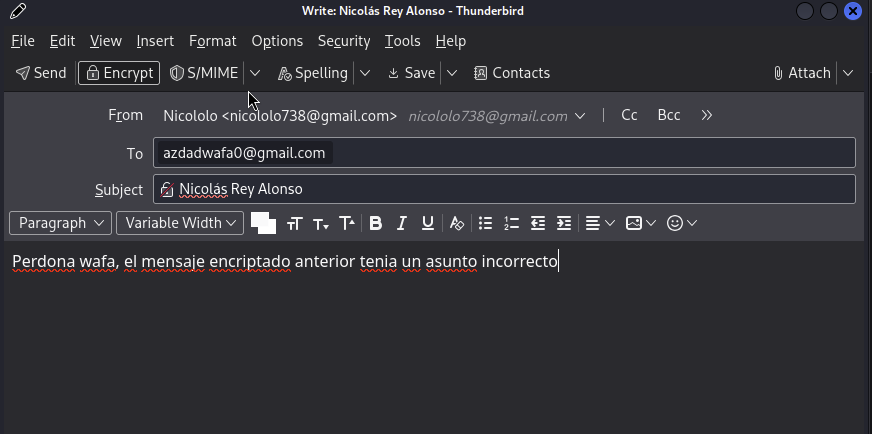
\includegraphics[width=\textwidth]{Imagenes/Mensaje_Encriptado_por_mi_thunderbird1.png}
    \caption{Composición de mensaje cifrado y firmado}
    \label{fig:msg_cifrado_1}
\end{figure}

\begin{figure}[H]
    \centering
    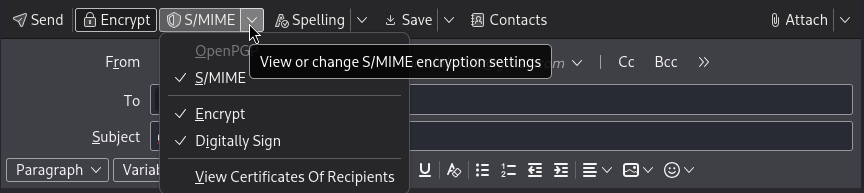
\includegraphics[width=\textwidth]{Imagenes/Mensaje_Encriptado_por_mi_thunderbird2.png}
    \caption{Mensaje cifrado y firmado enviado correctamente}
    \label{fig:msg_cifrado_2}
\end{figure}

\section{Recepción del mensaje cifrado y firmado de la compañera}

Recibimos el mensaje cifrado y firmado de Wafa Azdad Triki en Thunderbird. Se observa el adjunto \texttt{smime.p7m} que contiene el mensaje cifrado:

\begin{figure}[H]
    \centering
    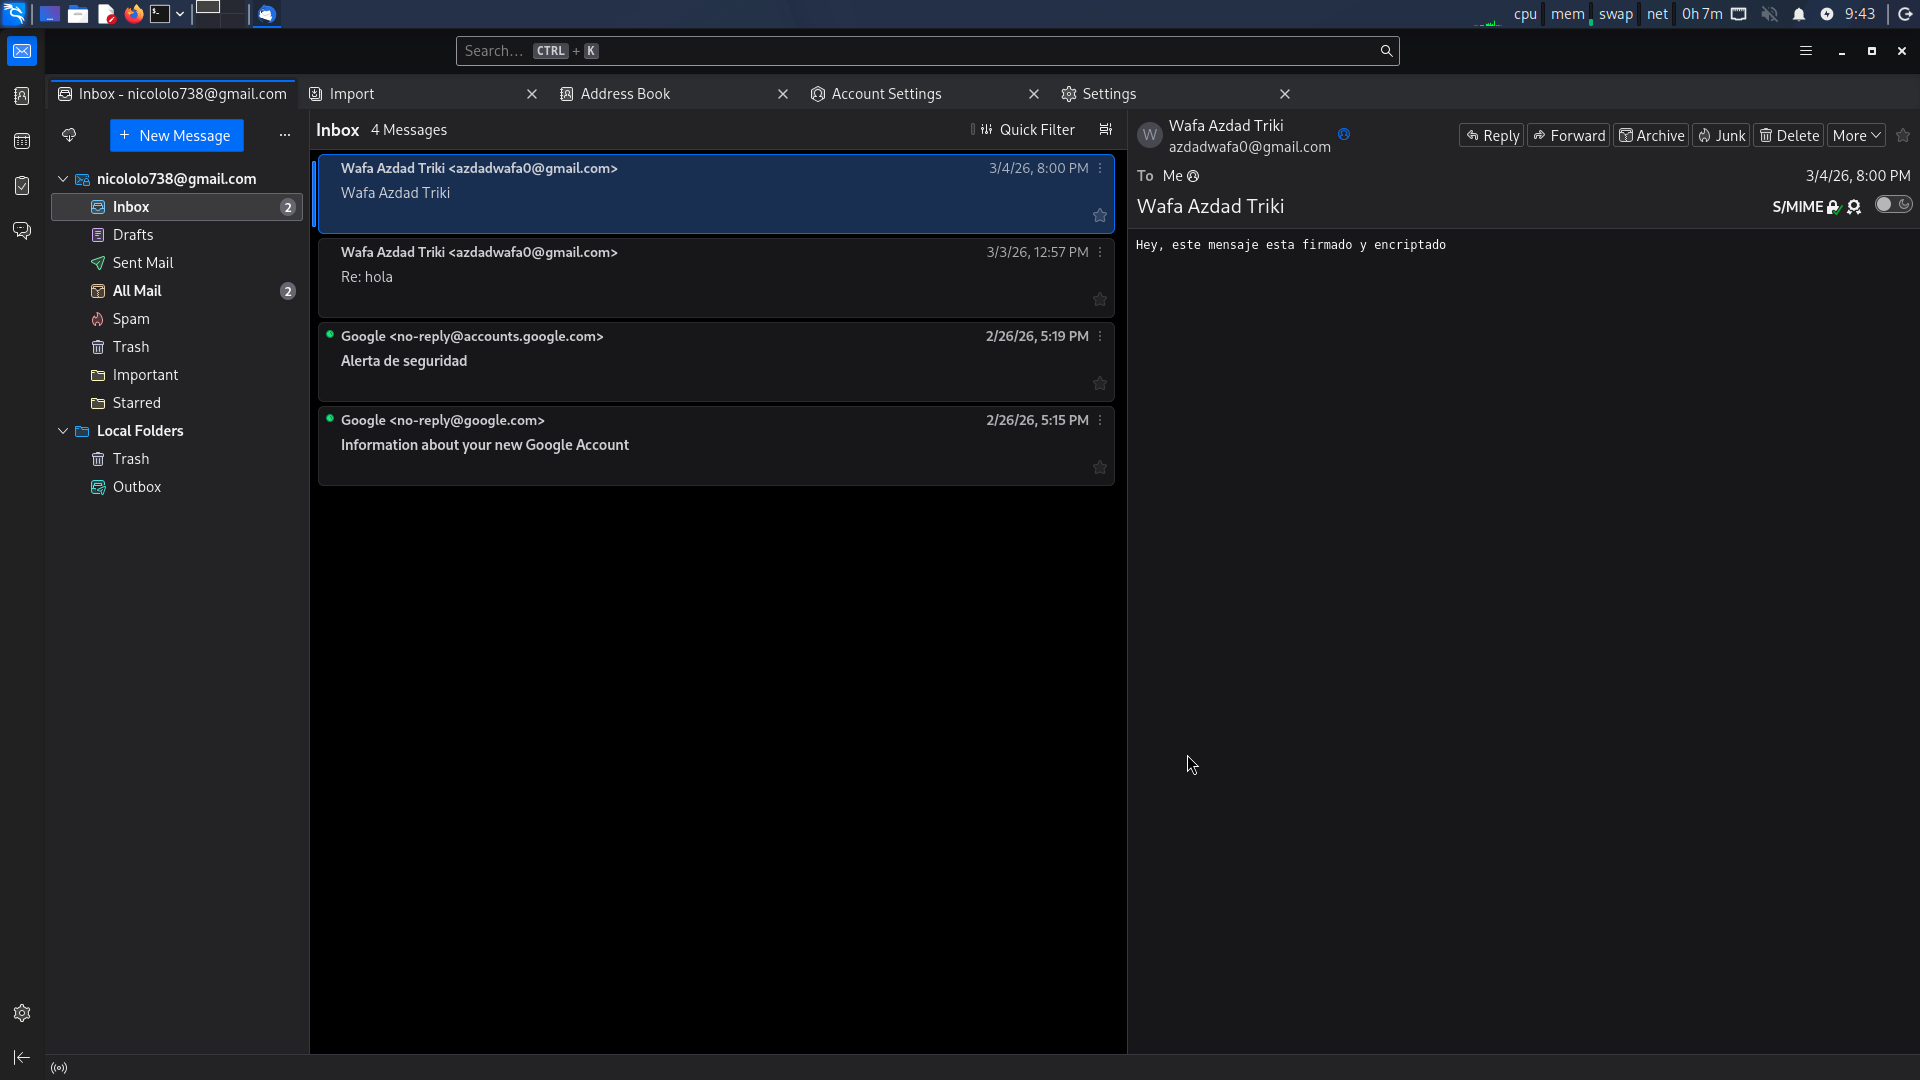
\includegraphics[width=\textwidth]{Imagenes/mensajecifradoencriptadoWafaEnThunderbird.png}
    \caption{Mensaje cifrado y firmado recibido de la compañera}
    \label{fig:msg_wafa_recibido}
\end{figure}

Para el procesamiento con OpenSSL, se guarda el mensaje completo en formato \texttt{.eml} (clic derecho $\rightarrow$ \textit{Guardar como\ldots}) y se exporta el certificado de la compañera en formato \texttt{.crt}:

\begin{figure}[H]
    \centering
    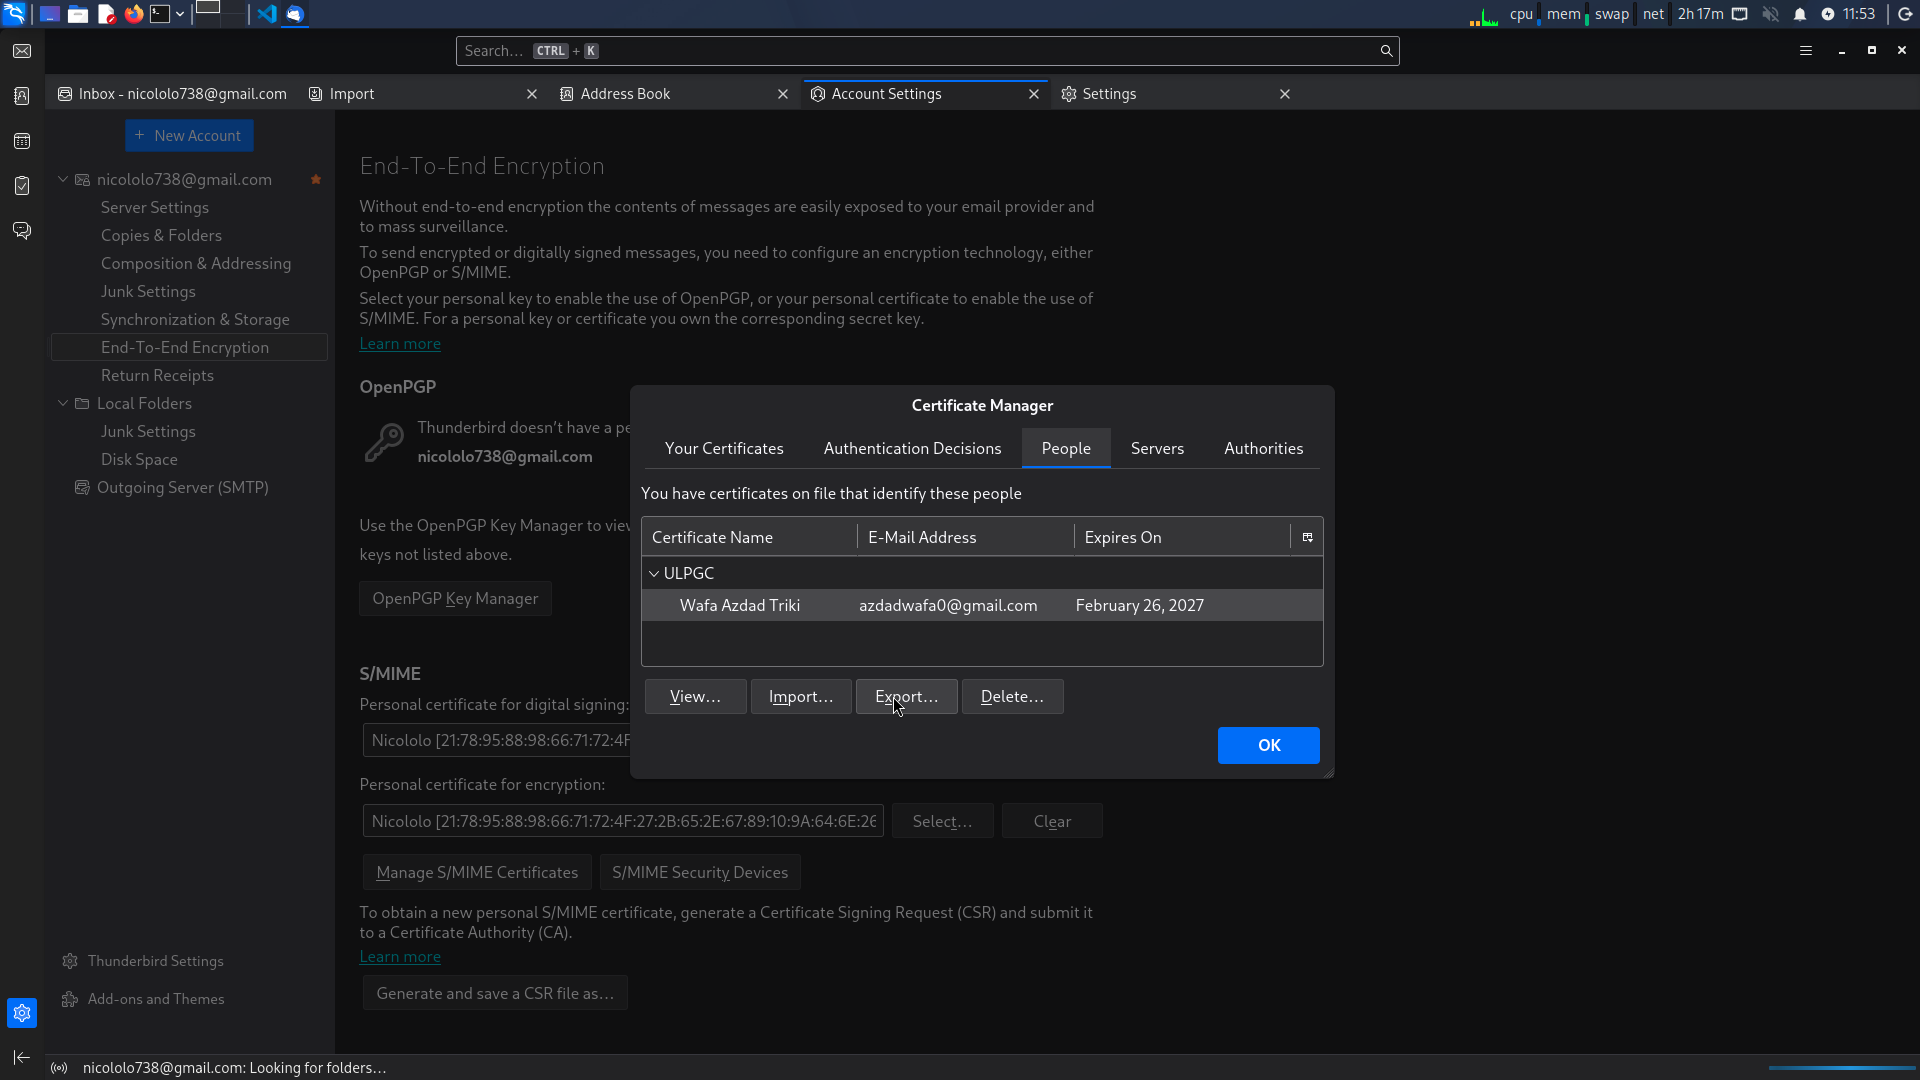
\includegraphics[width=\textwidth]{Imagenes/ExportarCertificadoWafaDeThunderbird.png}
    \caption{Exportación del certificado de la compañera desde Thunderbird}
    \label{fig:exportar_cert_wafa}
\end{figure}
